\documentclass[12pt]{article}

% packages

%\usepackage{times} % alt: cmbright
\usepackage[top=1in, bottom=1in, left=1in, right=1in]{geometry}
\usepackage{natbib}
\usepackage{amsmath}
\usepackage{amssymb}
\usepackage{latexsym}
\usepackage{sectsty}
\usepackage{amsfonts}
\usepackage{epsfig}
\usepackage{url}
\usepackage{microtype}
\usepackage{fixmath}
\usepackage{hyperref}
\usepackage{amsthm}
\usepackage{subfigure}
\usepackage{float}
\usepackage{hyperref}

\newtheorem{lem}{Lemma}
\newtheorem{defn}{Assumption}
\newtheorem{propty}{Property}
\newtheorem{thm}{Theorem}

% references

\newcommand{\mysec}[1]{Section~\ref{sec:#1}}
\newcommand{\myapp}[1]{Appendix~\ref{app:#1}}
\newcommand{\myeq}[1]{Equation~\ref{eq:#1}}
\newcommand{\myeqp}[1]{Eq.~\ref{eq:#1}}
\newcommand{\mychap}[1]{Chapter~\ref{chap:#1}}
\newcommand{\myfig}[1]{Figure~\ref{fig:#1}}

% math conveniences

\newcommand{\g}{\,\vert\,}
\newcommand{\E}{\textrm{E}}
\newcommand{\vct}[1]{\textbf{#1}}
\newcommand{\realline}{\mathbb{R}}
\newcommand{\indpt}{\protect\mathpalette{\protect\independenT}{\perp}}
\def\independenT#1#2{\mathrel{\rlap{$#1#2$}\mkern2mu{#1#2}}}
\newcommand{\h}[1]{\textrm{H}\left( #1 \right)}
\newcommand{\half}{\frac{1}{2}}
\newcommand{\new}{\textrm{new}}

\newcommand{\mult}{\textrm{Mult}}
\newcommand{\dir}{\textrm{Dir}}
\newcommand{\discrete}{\textrm{Discrete}}
\newcommand{\Bern}{\textrm{Bern}}
\newcommand{\DP}{\textrm{DP}}
\newcommand{\GP}{\textrm{GP}}
\newcommand{\Bet}{\textrm{Beta}}

% paragraph spacing

\setlength{\parindent}{0pt}
\setlength{\parskip}{2ex plus 0.5ex minus 0.2ex}

\allsectionsfont{\sffamily\mdseries}
\paragraphfont{\sffamily\bfseries}

\usepackage{algorithm}
\usepackage{algorithmic}
\renewcommand{\algorithmicrequire}{\textbf{Input:}}
\renewcommand{\algorithmicensure}{\textbf{Output:}}


\begin{document}

\title{\textsf{Semantic-Based Path Planning}}
\author{\textsf{Daqing Yi}}
\date{\textsf{Brigham Young University}}

\maketitle

\section{Semantic}

\begin{figure}
\centering
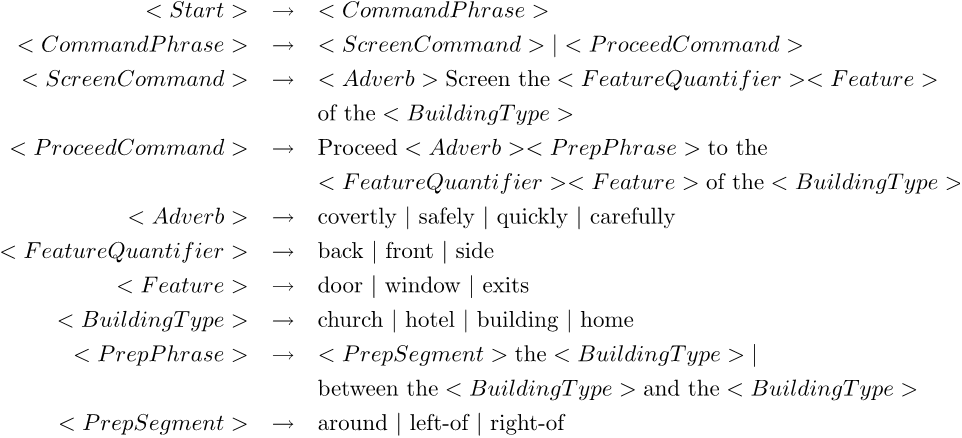
\includegraphics[width=0.7\linewidth]{./command}
\caption{An example of a command parser}
\label{fig:command}
\end{figure}

Fig.\ref{fig:command} defines a parser for a command format. $ <CommandPhrase> $ usually defines a task type. The domain of $ <BuildingType> $ and $ <Feature> $ are from predefined semantic labels. $ <PrepPhrase> $ and $ <FeatureQuantifier> $ gives the relationship with semantic labelled positions. $ <Adverb> $ rules the pattern of the trajectory.

Intuitively, the objectives in a command can be categorized into ``strong" and ``weak". Usually, the $ <BuildingType> $, $ <Feature> $ , $ <PrepPhrase> $ and $ <FeatureQuantifier> $ forms some ``strong" objectives. Implicitly, it expects an agent visiting some key positions defined from semantic. At the same time, $ <Adverb> $ shows ``weak" objective. It means with those key positions visited, the robot is expected to move in some expected pattern. Particularly, if a ``strong" objective violates a ``weak" objective, a ``strong" objective should be guaranteed. 




\section{Structure}

Assume the objectives inside a command can be divided into two types, we can import two key factors to a semantic-based path planning problem. One is ``waypoint" and the other is ``trajectory shape". ``waypoint" is used to satisfy the requirement on the constraint with semantic label, while ``trajectory shape" is determined by adverb.

I suggest to decompose the planning into two layers as in Fig.\ref{fig:planningLayer}, "waypoint layer" and ``spline layer".
\begin{itemize}
\item ``Waypoint layer" is the high layer, which is an abstract from smantic meaning of a command. It contains a sequence of waypoints that determines the coarse shape of a path. It can be presented in either discrete space or continuous space. This forms an abstract from semantic meaning of a command. 
\item ``Spline layer" is the lower layer is a set of splines connecting the waypoints by order. It generates the fine shape of each segment in the entire path. This layer is agent-dependent, how the shape is like depends on the task assigned to an agent and the capability of an agent. 
\end{itemize}

\begin{figure}
\centering
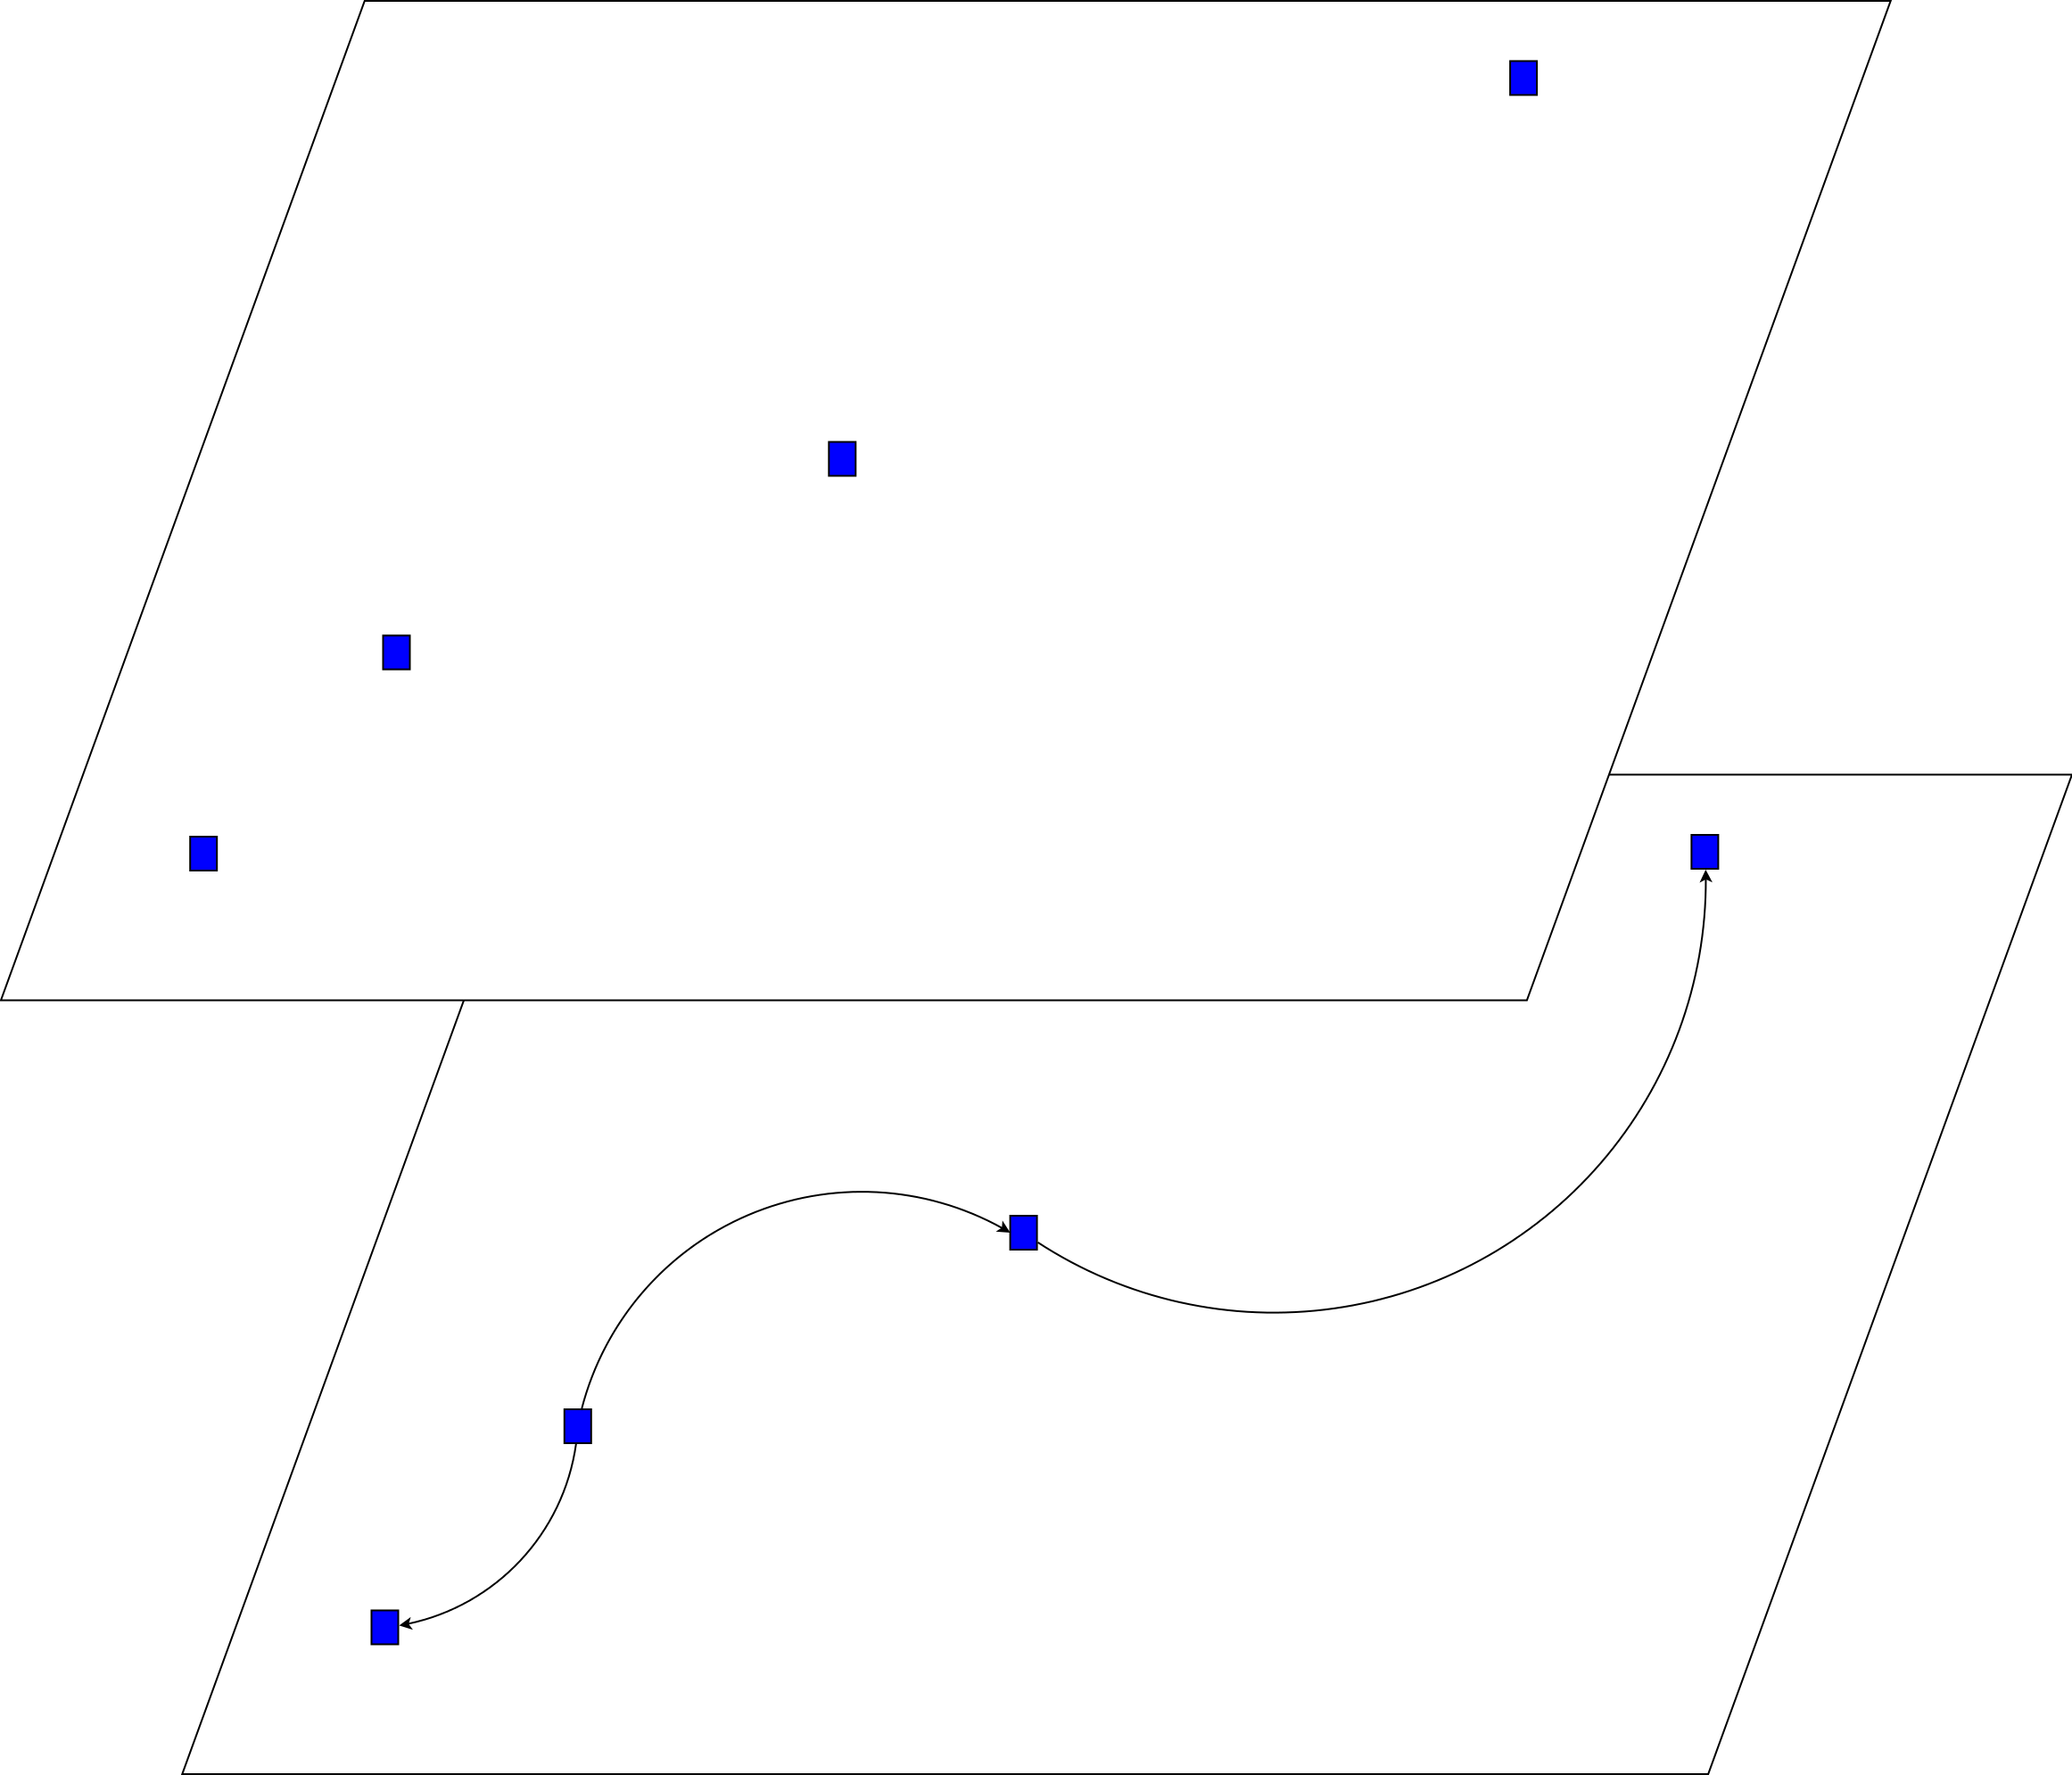
\includegraphics[width=0.4\linewidth]{./planningLayer}
\caption{Two Layers Planning Structure}
\label{fig:planningLayer}
\end{figure}

For example, if an robot is assigned to a search task and is required to reach to a specific position at some time. ``Waypoint layer" gives the key waypoints. Because the robot is still in the task of search, it will explore as large region as possible with considering on the maximum speed of the agent, which determines how the spline is like.

\section{Optimization}




\begin{enumerate}


\item \textbf{Walk through $ x_{1} $ and $ x_{2} $} \\
\label{obj:walk_through}
\textbf{Category:} Waypoint \\
\textbf{Domain:} Discrete/Continuous \\
\textbf{Comment:} A waypoint in between $ x_{1} $ and $ x_{2} $.


\item \textbf{Walk by $ x_{1} $} \\
\label{obj:walk_by}
\textbf{Category:} Waypoint \\
\textbf{Domain:} Discrete/Continuous \\
\textbf{Comment:} A waypoint in a tolerable range of $ x_{1} $. \\


\item \textbf{Shortest path} \\
\label{obj:short_path}
\textbf{Category:} Waypoint \\
\textbf{Domain:} Continuous \\
\textbf{Pre-Setup:} Generate visibility graph based on obstacles and find a sequence of nodes to connect start position with end position.

\item \textbf{Minimum visibility} \\
\label{obj:min_vis}
\textbf{Category:} Spline \\
\textbf{Type:} Objective Function \\
\textbf{Domain:} Discrete \\
\textbf{Pre-Setup:} Split the world into cells, calculate the visibility of each cell, $ visibility() $. \\
\textbf{Function:} $ \min \sum_{1}^{T} visibility(x^{t}) $ or $ \min \int visibility(x(t)) dt $. \\
\textbf{Comment:} \\

\item \textbf{Minimum exposure to dangerous area} \\
\label{obj:min_danger}
\textbf{Category:} Spline \\
\textbf{Type:} Objective Function \\
\textbf{Domain:} Discrete/Continuous \\
\textbf{Pre-Setup:} Having a distribution of dangerousness defined on the map, $ danger() $. \\
\textbf{Function:} $ \min \sum_{1}^{T} danger(x^{t}) $ or $ \min \int danger(x(t)) dt $. \\
\textbf{Comment:} minimize dangerousness accumulation in motion \\

\item \textbf{Get to a target position in shortest time} \\
\label{obj:pos_reach}
\textbf{Category:} Spline \\
\textbf{Type:} Objective Function \\
\textbf{Domain:} Discrete/Continuous \\
\textbf{Function:} $ \min \sum_{1}^{T} \parallel x^{t} - x^{target} \parallel $ or $ \min \int \parallel x(t) - x^{target} \parallel dt  $ \\
\textbf{Comment:} target driven motion \\

\item \textbf{Smooth motion curve} \\
\label{obj:min_curve}
\textbf{Category:} Spline \\
\textbf{Type:} Objective Function \\
\textbf{Domain:} Discrete/Continuous \\
\textbf{Function:} $ \min \sum_{1}^{T} \parallel orientation(x^{t}) - orientation(x^{t-1}) \parallel $ or $ \min \int \parallel \dot{x(t)} \parallel dt $.\\
\textbf{Comment:} move as smooth as possible \\

\item \textbf{Obstacle avoidance} \\
\label{obj:obs_avd}
\textbf{Category:} Spline \\
\textbf{Type:} Objective Function \\
\textbf{Domain:} Discrete/Continuous \\
\textbf{Function:} $ \min \sum_{1}^{T} \sum_{1}^{K} \parallel x^{t} - obstacle(k) \parallel $ or $ \min \int \sum_{1}^{K} \parallel x(t) - obstacle(k) \parallel dt $ \\
\textbf{Comment:} \\

\item \textbf{Collision avoidance} \\
\label{obj:col_avd}
\textbf{Category:} Spline \\
\textbf{Type:} Objective Function \\
\textbf{Domain:} Discrete/Continuous \\
\textbf{Function:} $ \min \sum_{1}^{T} \sum_{1}^{L} \parallel x^{t} - agent(l)^{t} \parallel $ or $ \min \int \sum_{1}^{L} \parallel x(t) - agent(l)^{t} \parallel dt $ \\
\textbf{Comment:} \\

\item \textbf{Information Maximization}
\label{obj:info_max}
\textbf{Category:} Spline \\
\textbf{Type:} Objective Function \\
\textbf{Domain:} Discrete/Continuous \\
\textbf{Pre-Setup:} 
\textbf{Function:}
\textbf{Comment:}   \\

\item \textbf{Not seen from particular locations} \\
\label{obj:not_seen}
\textbf{Category:} Spline \\
\textbf{Type:} Constraint \\
\textbf{Domain:} Discrete/Continuous \\
\textbf{Function:} $ \forall t, x^{t} \notin \bigcup_{j} visibility(z^{j}) $ \\
\textbf{Comment:} Remove the region that intersects with the visible regions of particular locations from the solution space. \\

\item \textbf{Wingman Constraint}
\label{obj:wingman}
\textbf{Category:} Waypoint/Spline \\
\textbf{Type:} Constraint \\
\textbf{Domain:} Discrete/Continuous \\
\textbf{Function:} $ \forall t, x^{t} \in wingmanArea(y^{t}) $ \\
\textbf{Comment:} Moving in a proximity of a human, $ y^{t} $ is the human position and $ wingmanArea() $ gives the wingman area by input position \\

\item \textbf{Avoid entering some place}
\label{obj:avd_enter}
\textbf{Category:} Waypoint/Spline \\
\textbf{Type:} Constraint \\
\textbf{Domain:} Discrete/Continuous \\
\textbf{Function:} $ \forall t, x^{t} \notin labelledRegion(s) $ \\
\textbf{Comment:} Avoiding of entering into some regions being semantically labelled. \\


\end{enumerate}

\section{Adverb}

\subsection{Covertly}
\begin{itemize}
\item Keeping avoid of being seen by others;
\item Smooth motion.
\end{itemize}
Relevant objectives:
Minimum visibility \ref{obj:min_vis}, Smooth motion curve \ref{obj:min_curve}

\subsection{Safely}
\begin{itemize}
\item Minmizing exposure to dangerous area;
\item Not seen from particular locations;
\end{itemize}
Relevant objectives:
Minimum exposure to dangerous area \ref{obj:min_danger}, Not seen from particular locations \ref{obj:not_seen}

\subsection{Quickly}
\begin{itemize}
\item Getting away from a position as quick as possible;
\item Getting close to a position as quick as possible;
\end{itemize}
Relevant objective:
Get to a target position in shortest time \ref{obj:short_path}

\subsection{Carefully} 
\begin{itemize}
\item Taking a steady and smooth motion so that people around will not be terrified; 
\item Being avoid of hitting anything or colliding with anybody;
\end{itemize}
Relevant objectives:
Smooth motion curve \ref{obj:min_curve}, Obstacle avoidance \ref{obj:obs_avd}, Collision avoidance \ref{obj:col_avd}

\subsection{Helpfully}
\begin{itemize}
\item Moving in a region near around a human.
\end{itemize}
Relevant objective:
Wingman Constraint \ref{obj:wingman}

\section{Example}

\textbf{``Proceed covertly and quickly between TMCB and HBLL along near the wall to the back door of HBLL"} \\
Here ``between TMCB and HBLL", ``along near the wall" and "to the back door of HBLL" shapes a sequence of waypoints. 
``Covertly" and ``quicky" give the spline patterns, which contain ``Minimum visibility", ``Smooth motion curve" and ``Get to a target position in shortest time".

\textbf{``Carefully and safely screen the park lot of TMCB"} \\
``The park lot of TMCB" returns a polygon from semantic labels, which generates a sequence of waypoints for screen task. 
``Carefully" and ``safely" give the spline patterns, which contain ``Smooth motion curve", ``Obstacle avoidance", ``Collision avoidance", ``Minimum exposure to dangerous area" and ``Not seen from particular locations".

\bibliographystyle{apalike}
\bibliography{bib}

\end{document}
